\documentclass{standalone}
\usepackage{tikz}
\usetikzlibrary{shapes.geometric, arrows}

\definecolor{mycolor}{RGB}{0, 153, 255}
\tikzstyle{process} = [rectangle, rounded corners,
                       minimum width=2cm, minimum height=1cm,
                       text centered, draw=black, fill=mycolor,
                       text=white, line width=0.3mm]

\tikzstyle{arrow} = [thick,->,>=stealth]

\begin{document}
    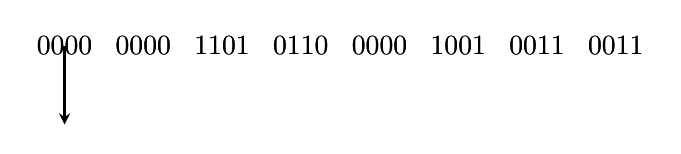
\begin{tikzpicture}[node distance=2cm]
        
        %32 bit instruction
        \node at (0,0) [text centered] (7) {0000};
        \node at (1,0) [text centered] (6) {0000};
        \node at (2,0) [text centered] (5) {1101};
        \node at (3,0) [text centered] (4) {0110};
        \node at (4,0) [text centered] (3) {0000};
        \node at (5,0) [text centered] (2) {1001};
        \node at (6,0) [text centered] (1) {0011};
        \node at (7,0) [text centered] (0) {0011};
        
        \draw [arrow] (0,0) -- (0,-1);
        
        %hex instrucion
        \node at (0,0) [text centered] (7) {0000};
        \node at (1,0) [text centered] (6) {0000};
        \node at (2,0) [text centered] (5) {1101};
        \node at (3,0) [text centered] (4) {0110};
        \node at (4,0) [text centered] (3) {0000};
        \node at (5,0) [text centered] (2) {1001};
        \node at (6,0) [text centered] (1) {0011};
        \node at (7,0) [text centered] (0) {0011};
        
    
    \end{tikzpicture}
\end{document}
